\documentclass[UTF8]{article}
\usepackage{ctex}
\usepackage{listings}
\usepackage[bf,small,indentafter,pagestyles]{titlesec} 

\usepackage{geometry}  %边距和纸张大小
\geometry{a4paper}
\geometry{left=2cm,right=2cm,top=3cm,bottom=3cm}
\usepackage{fancyhdr}
\usepackage{url}
 %使用graphicx包
\usepackage{graphicx}
\usepackage{amsmath}
\usepackage{amssymb} %使用数学符号使用 
\usepackage{cite} %使用引用 
\usepackage{enumerate} %使用item使用

\begin{document} 
\author{    彭峰     05121214   }
 \date{2015-5-10}
\title{忆阻}  %题目要改掉   后面
 \titlespacing{\chapter}{0pt}{*0}{*4}
\titlelabel{\S\thetitle\quad}
\maketitle%这是无目录只有title的部分

\section{前言}
先说说选题原因:还记得当年忆阻在实验室真正被实现时,我通过刊物了解到忆阻这一划时代的器件终于从理论转到实验阶段。还记得当时HP公司说希望在2012年实现成品进入市场。当时还很欣喜,说到时候就能用上这么高端的产品了,未想到现在还是处于实验室阶段,还在研究特性中。。随着大家对忆阻兴趣的提升,可以看到在设备架构、理论分析、理论模型和可能的应用上有大量的研究论文\cite{mem10}。为此查阅一定资料。

本次的选题实际上还是有较大的偏移的,忆阻作为第四种元件,虽然也可以当作有“记忆性能的电阻器”使用,但也应该和电阻和电容处于同一层次才是。想想这样和大家的选题不同,大家蜂拥至超级电容器也不是事,加之之前与忆阻的新闻有过一次邂逅,以前也有过了解,还是决定以“忆阻”为选题方向吧。

\section{背景介绍}
从中学和大学基础物理的书籍我们学习了三种主要元器件,分别是电阻,电容和电感,当然学习的时候多以线性元件为基础分析。1971年之前,华裔科学家蔡少棠发现在电流(i)、电压(v),电荷(q)及磁通量($\phi_{B}$)4种变量之间的6种关系有5种是已知的(图\eqref{fig:4})。
\begin{figure}[htbp]
\centering
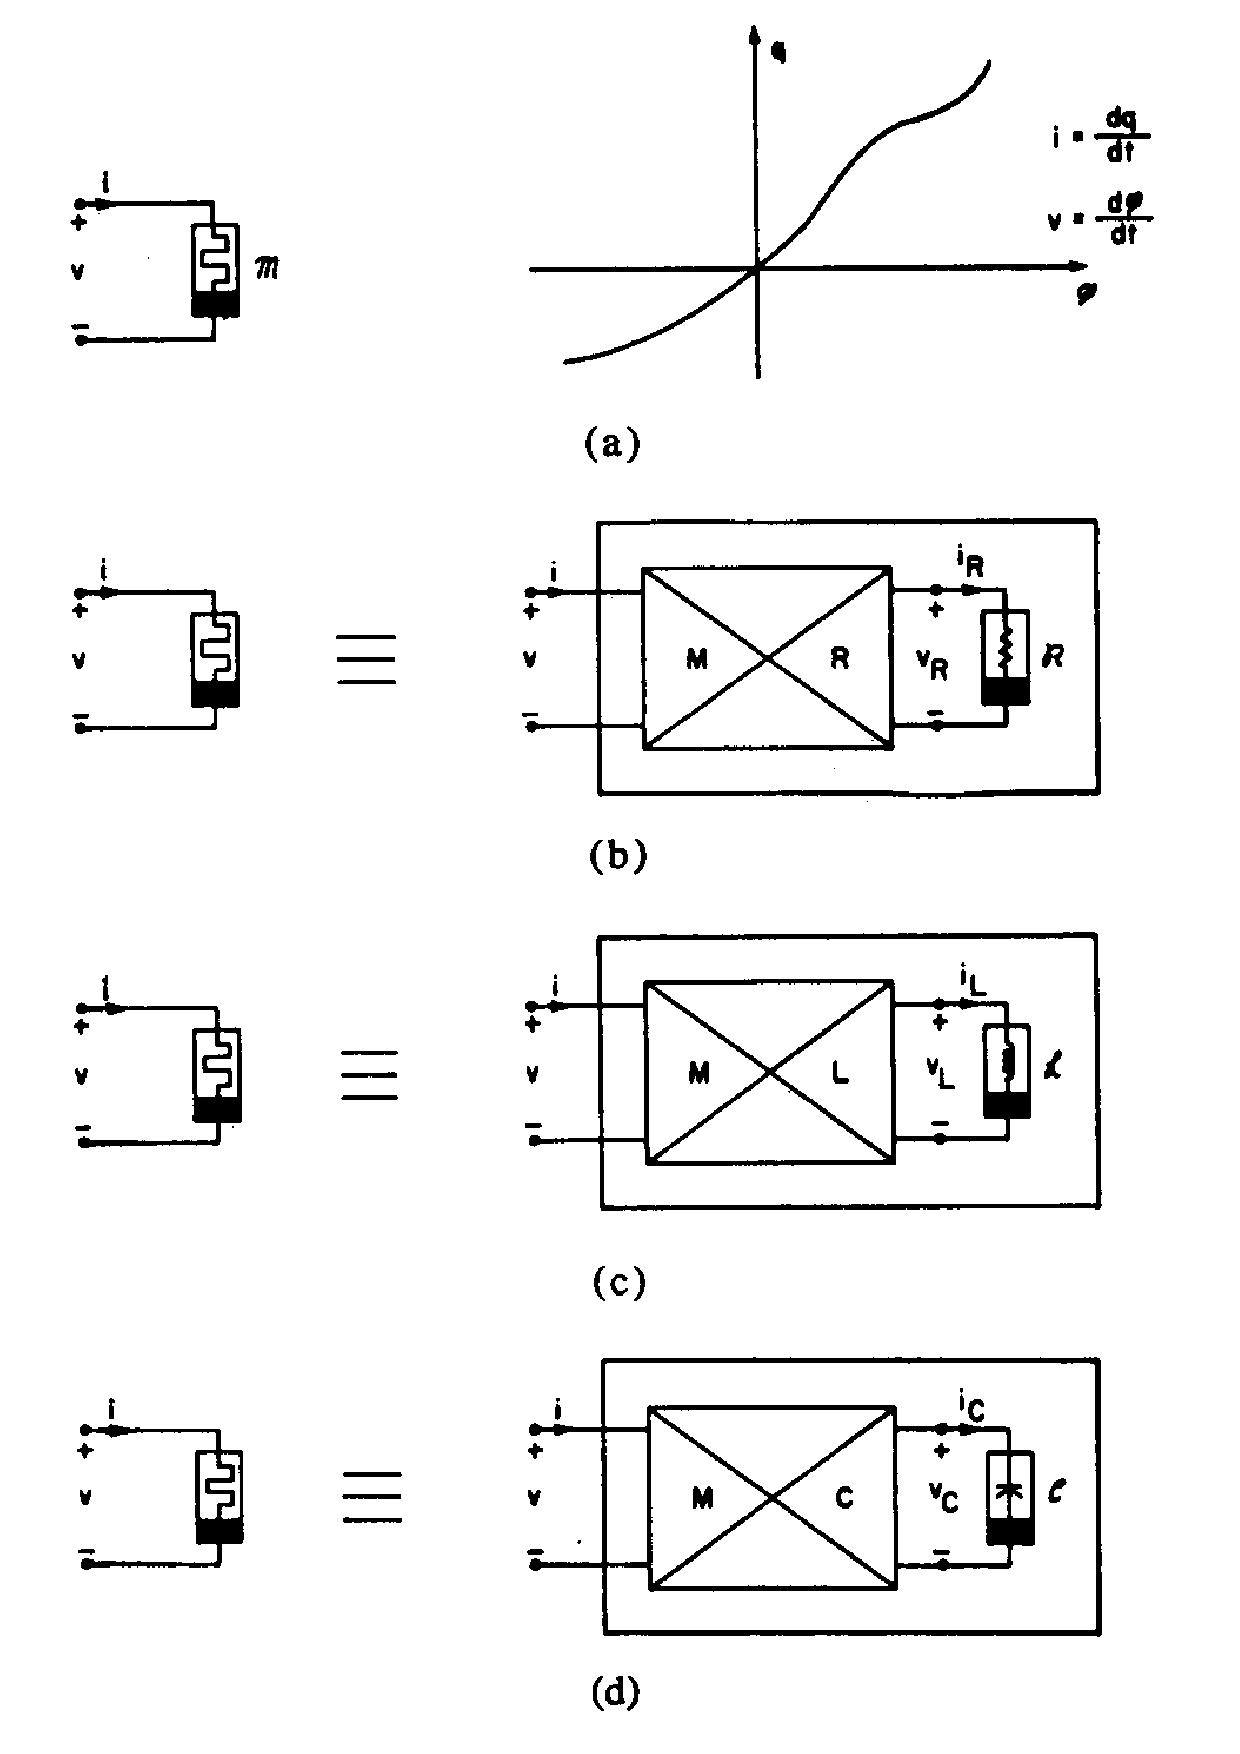
\includegraphics[width=3.42in,height=3in]{pic/4}
\caption{数学模型推想}
\label{fig:4}
\end{figure}

\subsection{忆阻理论的猜想和提出}
我们知道基于数学的自然理论是和谐的,所以他做了一系列的推断,通过外推对称的非线性电阻(电压与电流),非线性电容器(电压与电荷),和非线性电感(磁通量与电流)之间的的概念,猜想在电阻、电容和电感器之外,应该还有一种组件,代表着电荷与磁通量之间的关系\cite{mem00}。图\eqref{fig:m1}可以很好地展现四种基本元件的特征。
\begin{figure}[htbp]
\centering
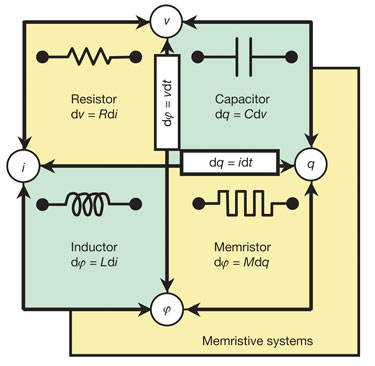
\includegraphics[width=2.12in,height=2.1in]{pic/memristor01.jpeg}
\caption{三大基本元件物理量关系}
\label{fig:m1}
\end{figure}
忆阻理论的提出很好的填补了四种基本物理量关系的空白。然而,这只是基于数学和谐性的猜想,虽然在当时蔡少棠通过普通的电子器件模拟了忆阻并且提出了相关性质,但是忆阻并没有真实在实验室实现。因此当时有人并不相信这种理论,认为这只是电阻和电感的一种结合方式,并不是存在。
事情的转机发生在2008年,HP在实验室偶然合成了这一器件。下面部分图片来自《How We Find Memsistor》一文。

\begin{figure}[htbp]
\centering
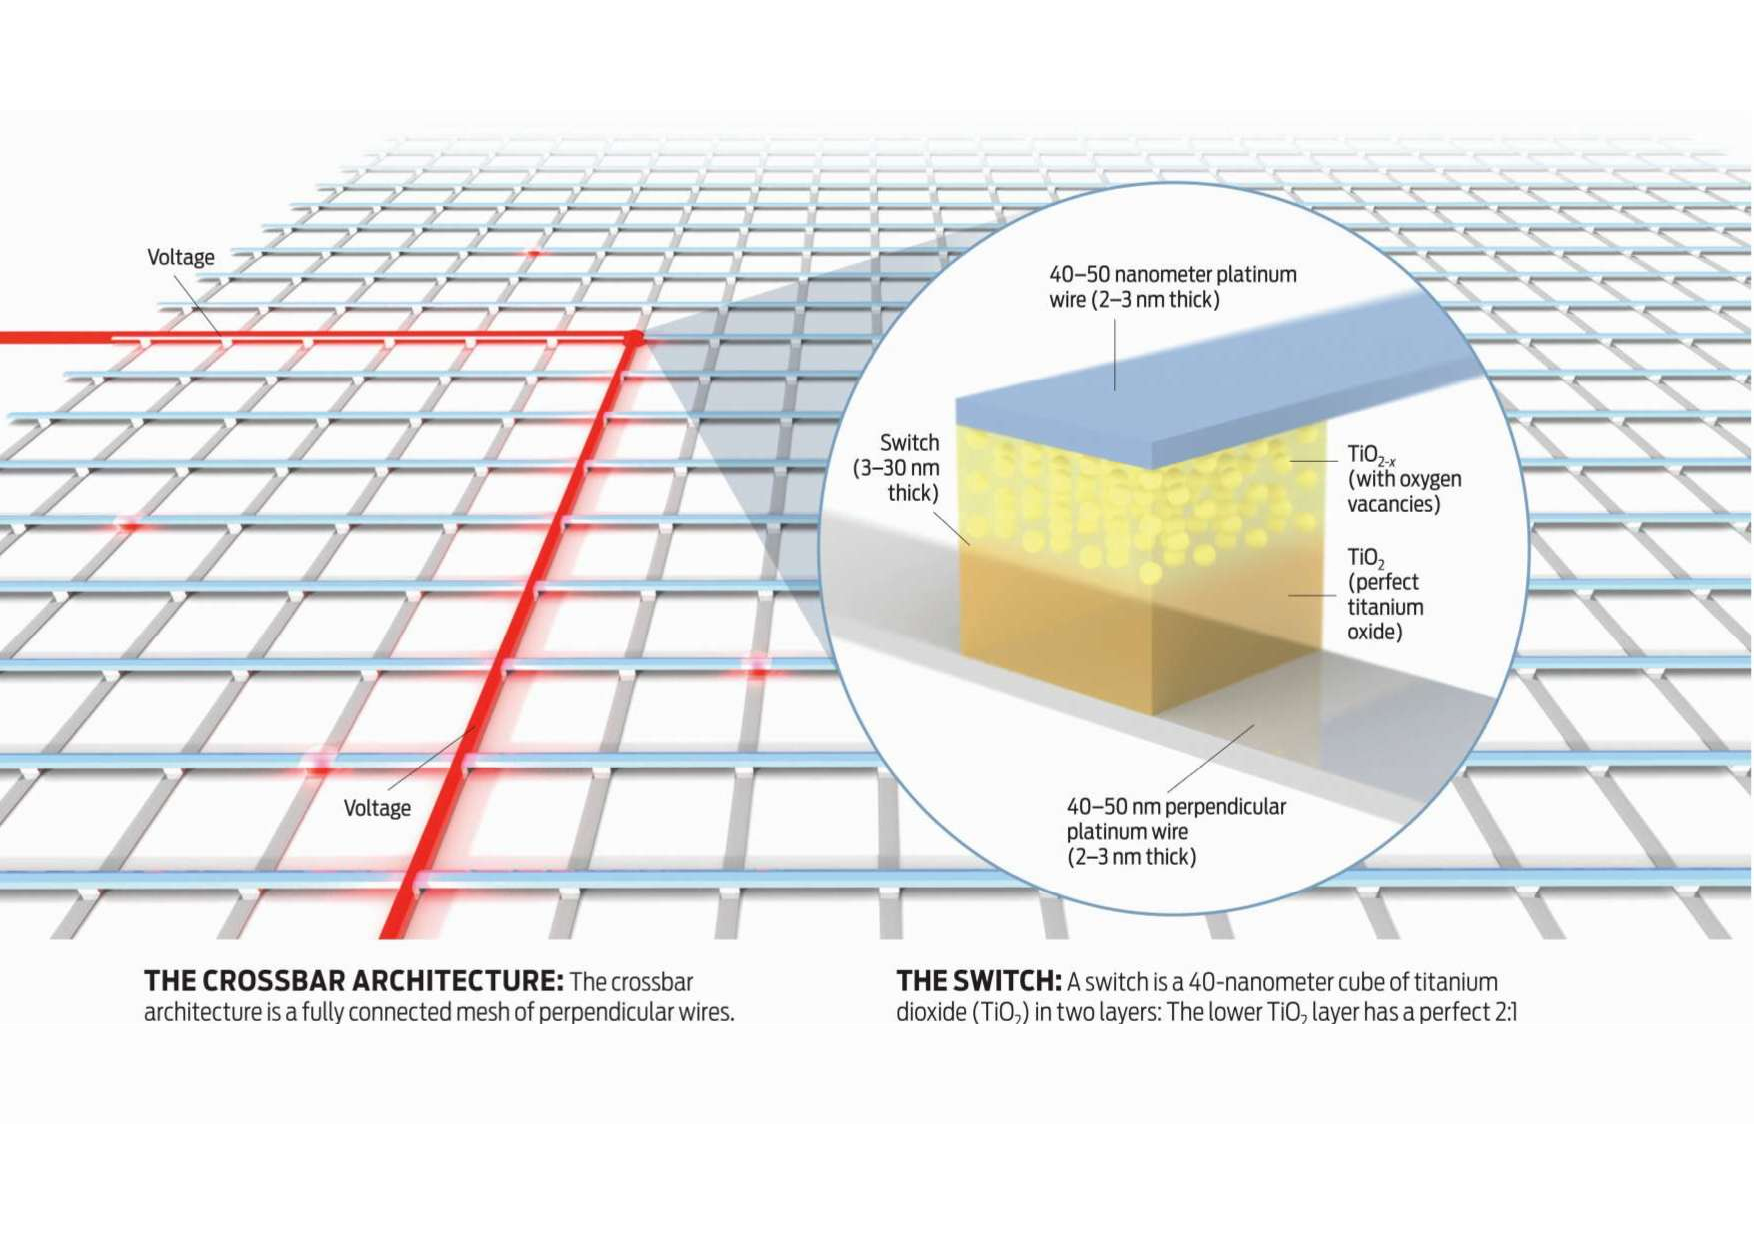
\includegraphics[width=5.77in,height=3.75in]{pic/71}
\caption{CrossBar Architecture}
\label{fig:71}
\end{figure}

\section{忆阻的发现}
%%下面多添加几个ref,,用moore定律的
从介绍上看,其忆阻的发现存在偶然性。上世纪90年代末,当时惠普公司高级研究员Stan Williams建立了该公司的信息和量子系统实验室,以便开拓未来20年的计算技术。40年来,工业界在经济驱动下不断制造基于摩尔定律的更小、更便宜的晶体管\cite{moore2}。于是,Williams研究团队开始研发越来越小的晶体管,这致使他们考虑当设备缩小到单个分子大小时会发生什么,以及单个原子运动将如何影响其性能。
%%%这个部分要看论文写!!


\subsection{CrossBar架构}
如图\eqref{fig:71}所示,
一排横向和一排纵向的电线组成的网格,在每一个交叉点上,放上一个「开关」连结一条横向和纵向的电线。让这两条电线控制这个开关的状态,当打开开关时,电压反转,关闭时,加上一个正向电压到对应的两根导线上。这样可以和计算机额的0、1相对应。意味着网格上的每一个交叉点都能储存一个位的数据。


\subsection{忆阻开关}
这是一个类似三明治的结构,由两根导线夹着40nm的钛的氧化物构成。最上方是纳米级的导线,中间部分是$TiO_{2}$层,内部包含游离的氧原子,下部是$TiO_{3}$层,内部原子结合较为稳定。最下方是又一根纳米数量级导线\cite{mem4}。
\begin{figure}[htbp]
\centering
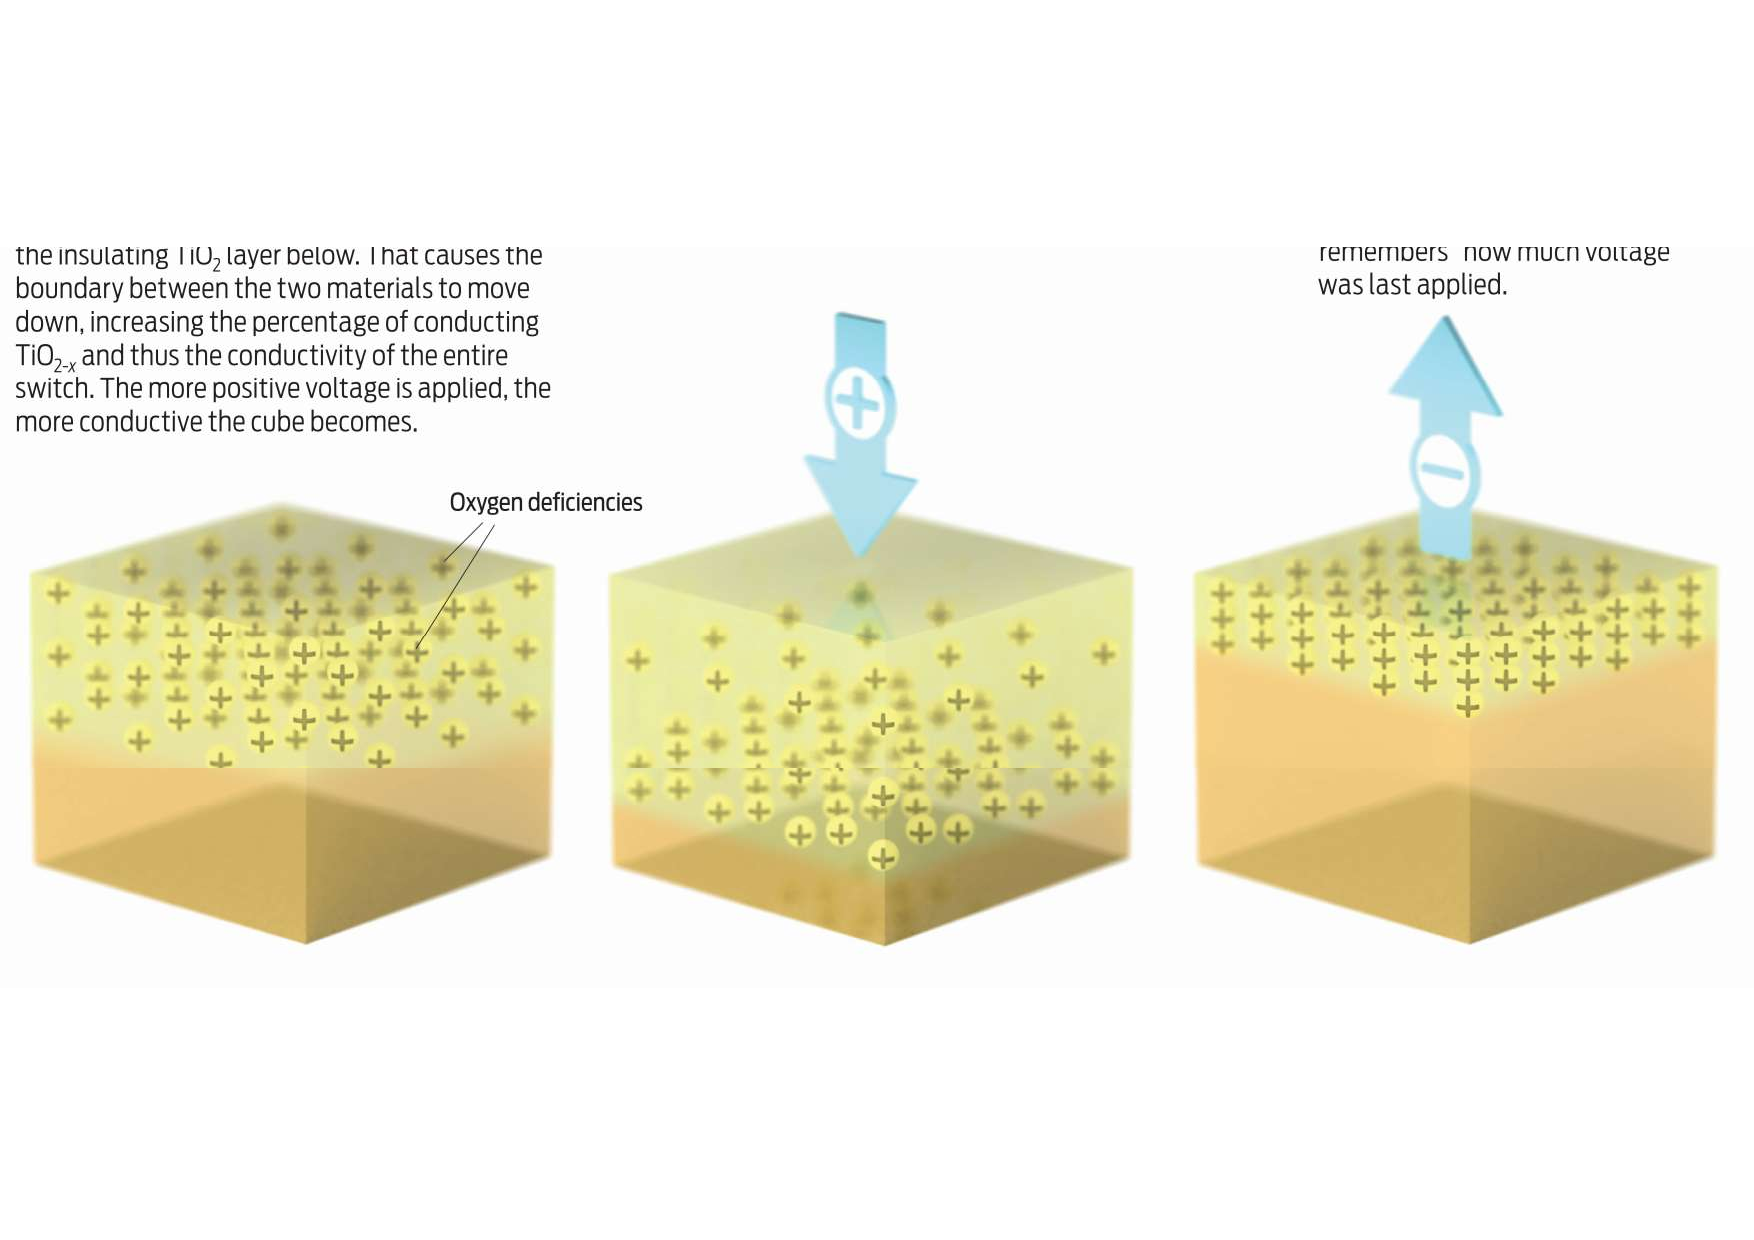
\includegraphics[width=5.77in,height=3.75in]{pic/8}
\caption{忆阻应用架构}
\label{fig:8}
\end{figure}
这一块极薄的二氧化钛被夹在两个电极中间,这
些二氧化钛又被分成两个部份,一半是正常的二氧化钛,另一半进行“掺杂”,使氧原子数减少。因此“掺杂”的那一半带正电,电流通过时电阻比较小,而且当电流从“掺杂”的一边通向正常的一边时,在电场的影响之下缺氧的“掺杂物”会逐渐往正常的一侧游移,使得以整块材料来言,“掺杂”的部份会占比较高的比重,整体的电阻也就会降低。反之,当电流从正常的一侧流向“掺杂”的一侧时,电场会把缺氧的“掺杂物”从回推,电阻就会跟着增加\cite{mem4}。


\section{忆阻的性质的探讨}

\subsection{忆阻的理论和性能}

%忆阻可以被制作的极其之小,但是可以完成晶体管的功能。通过使用特闷,我们能够制作~~~~~
忆阻器的特性--忆阻值M 满足式\eqref{eq:1}的特性:
\begin{equation}\label{eq:1}
M = \frac{\mathrm d\phi_{B}}{\mathrm dq}
\end{equation}

根据法拉第电磁感应定律及复合函数求导法则.对其积分,有:
\begin{equation}\label{eq:2}
M(q(t)) = \frac{\int\mathnormal{v(t)dt}}{\int\mathnormal{i(t)dt}}
\end{equation}
由式\eqref{eq:2}可以看出,忆阻的值和电阻有着相同的量纲,但是其阻值取决于过去流过的电荷的总量,即忆阻有着记忆特性,且在断电状态下保持不变。这和电容器的电压比较类似。

%R(I)=\frac{\mathrm dV}{\mathrm dI}
我们用一个表格来看下忆阻器的和其他元器件的对比:

\begin{tabular}{|c|c|c|}

\hline
& 电荷(q)& 电流(I) \\

 \hline
电压(U)  & 电容(倒数) &电阻率 \\
     & $\frac{1}{C}=\frac{\mathrm{d}U}{\mathrm{d}q}=\frac{\mathrm{d}\dot \Phi}{\mathrm{d}q}$  &   $R=\frac{\mathrm{d}U}{\mathrm{d}I}=\frac{\mathrm{d}\dot \Phi}{\mathrm{d}\dot{q}}$ \\
 \hline
磁通量($\Phi$)  & 忆阻器 & 电感 \\
     & $M=\frac{\mathrm{d}\Phi}{\mathrm{d}q}$  &  $L=\frac{\mathrm{d}\Phi}{\mathrm{d}I}=\frac{\mathrm{d}\Phi}{\mathrm{d}\dot{q}}$ \\
 \hline
\end{tabular}


\subsection{模型解释}
这里对图\eqref{fig:8}进行一个简单分析,掺杂了氧空位的氧化钛 层电阻较小,纵横 闩中掺杂层所占比例较大,纵横闩处于导通状态 ;无掺杂氧空 位的氧化钛层 电阻较大,纵横闩中无掺杂层所 占比例较大,纵横闩处于断路状 态。纵横闩的电阻可以简单的看做是掺杂部分 电阻和无掺杂部分的电阻之和。 令纵横闩的总厚度为D,掺杂层的即时厚度为$\mathnormal{w(t)}   $,若纵横闩全部为掺杂层 , 总电阻记为$R_{ON}$ ,那么掺杂层的即时电阻为$R_{ON} \frac{\mathnormal{w_{t}}}{\mathnormal{D}}$。若纵横闩全部为无掺杂 层,总电阻记为$R_{OFF}$ ,无掺杂层的即时电阻为$R_{OFF}(1 - \frac{w_{t}}{D})$。当忆阻器电极施 加偏置电压$v(t)$,忆阻器内部会导致离子迁移\cite{mem2013}。设在理 欧姆接触及线性的 电子迁移的情况下,离子迁移率为$\mu_{\gamma}$
\begin{equation}\label{eq:model1}
v_{t} = (R_{ON} \frac{w_{t}}{D} + R_{OFF}(1 - \frac{w_{t}}{D}) ) i(t)
\end{equation}
\begin{equation}\label{eq:model2}
\frac{dw(t)}{dt} = \mu_{\gamma}\frac{R_{ON}}{D}q(t)
\end{equation}

两式\eqref{eq:model1}\eqref{eq:model2}很好的满足了忆阻数学特性模型图\eqref{eq:1}图\eqref{eq:2}


\begin{figure}[htbp]
\centering
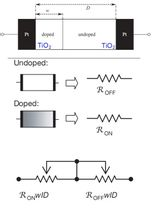
\includegraphics[width=2.77in,height=1.75in]{pic/no2.jpeg}

\caption{等效器件}
\label{fig:graph}
\end{figure}


%\subsection{忆阻的疑惑}
%%%提出记忆电阻,记忆电容和记忆电感三种理论


%\section{目前忆阻应用的地方(改题目)}  改现状与未来
%%%记得那个部分的提出就放这个地方
\section{忆阻的现状与未来}
毫无疑问忆阻作为重新证实的基本器件在未来会发挥出良好的前景,然而目前还是处于实验室阶段,对其的认知和性质了解还是不够,这限制了忆阻的一步使用。
目前应用的 地方主要在人工智能和神经网络上\cite{mem2009},通过混合型电路-包含大量相连的忆阻和电阻,可以更好的辨识人类的具体的行为模式,这正是目前计算机所不能达到的。像可快速获取的在人流中的人脸识别。
同时由于高密度的优势,每平方英寸能存储的容量极大,加之可以进行堆栈的3D构成,可以见到是存储的一种绝佳替代品\cite{mem2012}。2012年,HRL实验室(一个由通用汽车公司和波音公司共有的研究设施)宣布首次成功运行忆阻器阵列\cite{mem2010},即利用了用于电子设备生产的互补金属氧化物半导体(CMOS)制造工艺。澳大利亚墨尔本皇家理工大学 的科学家用非晶 钙钛矿氧化物开发出一种纳米级超快忆阻器\cite{ou},采用了一种纳米级的薄膜材料来制 造忆阻器 ,这种 功能性氧化物 比人类 头发的直径薄 1 000倍 。这种材料 在化学 上具有 “忆 阻”效应 ,存储 在其 中的数 据具有非易失性 。 受到经济和材料的影响,各大公司在对摩尔定律的追求已经开始放缓,相信新型基本器件的发现可以再一次带来工业界的革命\cite{moore1},


\bibliography{end}
\bibliographystyle{plain}





\end{document}

